\chapter{Bioinformatics Fundamentals}
\label{ch:bioinfofundamentals}

\begin{sourcebox}
The alignment and file-processing foundations are anchored by the BWA and SAMtools papers \cite{li2009bwa,li2009}. File-format authority ultimately lies in the current specification, while command behavior lies in the named software release and its help text.
\end{sourcebox}

\begin{keyconcept}
Bioinformatics is the interdisciplinary field that develops and applies computational methods to analyse, interpret, and manage biological data---particularly the vast quantities of sequence data generated by modern \acrshort{NGS} platforms. Mastering bioinformatics fundamentals is essential for any researcher who generates or analyses sequencing data: without appropriate computational tools and practices, even the highest-quality sequencing data cannot be translated into biological insight.
\end{keyconcept}

\section{What Is Bioinformatics?}
\label{sec:bioinf:what}

At its core, bioinformatics sits at the intersection of biology, computer science, mathematics, and statistics. It encompasses the development of algorithms and software tools for processing raw sequencing data (alignment, quality control, variant calling), the design of databases and ontologies for organising biological knowledge, and the application of statistical and machine-learning methods for extracting meaningful patterns from high-dimensional datasets.

For the genomics practitioner, bioinformatics is not a separate discipline but an integral part of every sequencing experiment. The moment reads leave the sequencer, the project becomes a computational endeavour. Understanding the computing environment, file formats, key tools, programming languages, and workflow management systems described in this chapter is therefore a prerequisite for every subsequent analysis chapter in this book.

%=============================================================================
\section{Computing Environment Setup}
\label{sec:bioinf:computing}
%=============================================================================

\subsection{Linux/Unix Basics for Bioinformatics}
\label{subsec:bioinf:linux}

Nearly all bioinformatics software is developed for, and best supported on, Linux and Unix-like operating systems. Even researchers who use macOS or Windows on their personal machines will typically run analyses on a Linux-based high-performance computing (HPC) cluster or cloud instance. The command-line interface (CLI) is the primary means of interaction.

Essential command-line skills include:

\begin{itemize}[itemsep=2pt]
  \item \textbf{Navigation:} \texttt{cd}, \texttt{ls}, \texttt{pwd}, \texttt{tree}.
  \item \textbf{File manipulation:} \texttt{cp}, \texttt{mv}, \texttt{rm}, \texttt{mkdir}, \texttt{ln -s} (symbolic links).
  \item \textbf{Text processing:} \texttt{cat}, \texttt{head}, \texttt{tail}, \texttt{less}, \texttt{wc}, \texttt{grep}, \texttt{sed}, \texttt{awk}, \texttt{cut}, \texttt{sort}, \texttt{uniq}.
  \item \textbf{Compression:} \texttt{gzip}/\texttt{gunzip}, \texttt{bgzip} (block-gzip for indexed access), \texttt{zcat}.
  \item \textbf{Pipes and redirection:} combining commands with \texttt{|}, \texttt{>}, \texttt{>>}, \texttt{2>}.
  \item \textbf{Process management:} \texttt{top}/\texttt{htop}, \texttt{ps}, \texttt{kill}, \texttt{nohup}, \texttt{screen}/\texttt{tmux}.
  \item \textbf{Permissions:} \texttt{chmod}, \texttt{chown}; understanding \texttt{rwx} triplets.
  \item \textbf{Environment variables:} \texttt{export}, \texttt{PATH}, \texttt{.bashrc}/\texttt{.bash\_profile}.
\end{itemize}

\begin{tipbox}[title={Screen and Tmux}]
Use \texttt{screen} or \texttt{tmux} to create persistent terminal sessions on remote servers. If your SSH connection drops during a long-running job, the process continues safely inside the session. This is indispensable for interactive bioinformatics work on HPC clusters.
\end{tipbox}

\begin{lstlisting}[language=bash,caption={Essential Linux commands for bioinformatics.},label=lst:linux-basics]
# Count reads in a FASTQ file (4 lines per read)
wc -l sample.fastq | awk '{print $1/4}'

# Extract chromosome 1 alignments from a BAM file
samtools view -b input.bam chr1 > chr1.bam

# Sort a BED file and merge overlapping intervals
sort -k1,1 -k2,2n peaks.bed | bedtools merge > merged.bed

# View the first few records of a gzipped VCF
zcat variants.vcf.gz | grep -v "^#" | head -20

# Monitor disk usage of a project directory
du -sh /data/project/*
\end{lstlisting}

\subsection{Package Managers}
\label{subsec:bioinf:packagemanagers}

Installing bioinformatics software can be challenging due to complex dependency chains. Modern package managers greatly simplify this process:

\begin{description}[style=nextline, font=\bfseries, itemsep=4pt]
  \item[Conda / Mamba]
  Conda is the most widely used package manager in bioinformatics. It manages both software binaries and their dependencies within isolated \textit{environments}, preventing version conflicts between projects. The \texttt{bioconda} channel provides over 11,000 bioinformatics packages. \texttt{Mamba} is a drop-in replacement for \texttt{conda} with significantly faster dependency resolution.

  \item[Pip]
  Python's native package manager. Used for Python-specific packages not available through Conda (e.g., niche libraries on PyPI). Best used \textit{within} a Conda environment to avoid conflicts with system Python.

  \item[Bioconductor]
  The primary repository for R-based bioinformatics packages. Bioconductor provides a curated, versioned ecosystem of packages for genomic data analysis, including \software{DESeq2}, \software{edgeR}, \software{GenomicRanges}, and hundreds of others. Packages are installed via \texttt{BiocManager::install()}.
\end{description}

\begin{lstlisting}[language=bash,caption={Setting up a Conda environment for bioinformatics.},label=lst:conda-setup]
# Install Miniforge (includes mamba)
curl -L -O https://github.com/conda-forge/miniforge/releases/latest/download/Miniforge3-Linux-x86_64.sh
bash Miniforge3-Linux-x86_64.sh

# Create an environment for an RNA-seq project
mamba create -n rnaseq -c conda-forge -c bioconda \
  fastqc=0.12.1 fastp=0.23.4 star=2.7.11b \
  subread=2.0.6 samtools=1.19 multiqc=1.21

# Activate the environment
mamba activate rnaseq

# Export the environment for reproducibility
mamba env export > environment.yml
\end{lstlisting}

\subsection{Containers: Docker and Singularity/Apptainer}
\label{subsec:bioinf:containers}

Containers provide a higher level of reproducibility than package managers by encapsulating the entire software environment---operating system libraries, tools, and configuration---into a portable, immutable image.

\begin{description}[style=nextline, font=\bfseries, itemsep=4pt]
  \item[Docker]
  The most widely used container platform. Docker images are available for virtually every bioinformatics tool (e.g., on Docker Hub or Quay.io). Docker requires root privileges to run, which limits its use on shared HPC clusters.

  \item[Singularity / Apptainer]
  Designed for HPC environments where users do not have root access. Singularity (now rebranded as Apptainer) can run Docker images directly without modification. Most HPC centres support Singularity/Apptainer.
\end{description}

\begin{lstlisting}[language=bash,caption={Using containers for bioinformatics.},label=lst:containers]
# Pull and run a Docker image for FastQC
docker pull biocontainers/fastqc:v0.12.1
docker run --rm -v $(pwd):/data biocontainers/fastqc:v0.12.1 \
  fastqc /data/sample_R1.fastq.gz /data/sample_R2.fastq.gz

# On HPC: convert Docker image to Singularity/Apptainer
singularity pull docker://biocontainers/fastqc:v0.12.1
singularity exec fastqc_v0.12.1.sif fastqc sample_R1.fastq.gz

# BioContainers provides images for most bioinformatics tools
# See: https://biocontainers.pro
\end{lstlisting}

\begin{keyconcept}[title={Containers for Reproducibility}]
A Conda environment specifies what software to install; a container specifies the exact binary files, libraries, and operating system state. Containers provide ``bit-for-bit'' reproducibility---the same container will produce identical results on any machine, even years later. For published analyses, containers are the gold standard for computational reproducibility.
\end{keyconcept}

\subsection{HPC Clusters: SLURM, PBS/Torque, SGE}
\label{subsec:bioinf:hpc}

Most bioinformatics analyses require computational resources beyond what a laptop or desktop can provide. High-performance computing (HPC) clusters provide shared pools of CPUs, RAM, and storage. Jobs are submitted through a \textbf{workload manager} (also called a job scheduler):

\begin{description}[style=nextline, font=\bfseries, itemsep=3pt]
  \item[SLURM (Simple Linux Utility for Resource Management)]
  The most widely deployed scheduler in academic HPC. Jobs are submitted with \texttt{sbatch}, monitored with \texttt{squeue}, and cancelled with \texttt{scancel}.

  \item[PBS/Torque]
  An older but still common scheduler. Jobs are submitted with \texttt{qsub} and monitored with \texttt{qstat}.

  \item[SGE (Sun Grid Engine) / Open Grid Scheduler]
  Legacy scheduler found in some older installations. Also uses \texttt{qsub}/\texttt{qstat} syntax.
\end{description}

\begin{lstlisting}[language=bash,caption={SLURM job submission for a bioinformatics task.},label=lst:slurm]
#!/bin/bash
#SBATCH --job-name=bwa_align
#SBATCH --output=logs/bwa_%j.out
#SBATCH --error=logs/bwa_%j.err
#SBATCH --cpus-per-task=16
#SBATCH --mem=32G
#SBATCH --time=06:00:00
#SBATCH --partition=standard

# Load modules or activate environment
source activate wgs_pipeline

# Run BWA-MEM2 alignment
bwa-mem2 mem -t 16 \
  /ref/GRCh38.fa \
  sample_R1.fastq.gz sample_R2.fastq.gz \
  | samtools sort -@ 4 -o sample.sorted.bam -

samtools index sample.sorted.bam
\end{lstlisting}

\subsection{Cloud Computing for Genomics}
\label{subsec:bioinf:cloud}

Cloud computing offers elastic, on-demand computational resources without the capital investment of purchasing hardware. The three major cloud providers each offer genomics-specific services:

\begin{itemize}[itemsep=3pt]
  \item \textbf{Amazon Web Services (AWS):} AWS HealthOmics for managed genomics workflows; S3 for storage; EC2 for compute; AWS Batch for job scheduling. The Registry of Open Data on AWS hosts public genomics datasets (1000 Genomes, TCGA, gnomAD).
  \item \textbf{Google Cloud Platform (GCP):} Google Cloud Life Sciences API; BigQuery for large-scale variant analysis; Terra platform (Broad Institute) for WDL-based workflows running on GCP.
  \item \textbf{Microsoft Azure:} Azure Genomics; Cromwell on Azure for WDL workflows; integration with Microsoft's healthcare data solutions.
\end{itemize}

\begin{warningbox}[title={Cloud Cost Management}]
Cloud computing can become expensive if not carefully managed. A single misconfigured pipeline can generate thousands of dollars in compute charges within hours. Always set budget alerts, use spot/preemptible instances for fault-tolerant workloads (50--80\% cost savings), and shut down instances when not in use. Estimate costs before running large analyses using the provider's pricing calculators.
\end{warningbox}

%=============================================================================
\section{Bioinformatics File Formats}
\label{sec:bioinf:formats}
%=============================================================================

A thorough understanding of file formats is essential for working with sequencing data. Each format serves a specific purpose in the analysis pipeline, and knowing their structure helps in debugging problems and writing custom analyses.

\subsection{FASTA: Reference Sequences}
\label{subsec:bioinf:fasta}

The FASTA format is one of the simplest and oldest bioinformatics formats, used to store nucleotide or protein sequences. Each record consists of a header line beginning with \texttt{>} followed by one or more lines of sequence:

\begin{lstlisting}[caption={FASTA format example.},label=lst:fasta]
>chr1 Homo sapiens chromosome 1
NNNNNNNNNNNNNNNNNNNNNNNNNNNNNNNNNNNNNNNNNNNNNNNNNN
NNNNNNNNNNNNNNNNNNNNNNNNNNNNNNGATAATCTACTACTACTCAG
TGGCCAACACCTGATCCTGACAGCTGGAGTAAGGAACCTGAAGTCCCTA
AAACTCATCAATGTTCTTTAGAGACTTACCAGGACCACTTCGTGAGGGA
>chr2 Homo sapiens chromosome 2
NNNNNNNNNNNNNNNNNNNNNNNNNNNNNNNNNNNNNNNNNNNNNNNNNN
AGAGATCAGCTCAGGAGAGTCTCTTGAAGAAATCTGATTCACTGTATGG
\end{lstlisting}

Reference genomes (e.g., GRCh38/hg38 for human) are distributed in FASTA format. For efficient random access, FASTA files are indexed with \texttt{samtools faidx}, producing a \texttt{.fai} index file. Many tools also require a sequence dictionary (\texttt{.dict}) created with \software{Picard} or \software{samtools}.

\subsection{FASTQ: Raw Sequencing Reads}
\label{subsec:bioinf:fastq}

FASTQ is the universal output format for sequencing instruments. Each read consists of exactly four lines:

\begin{lstlisting}[caption={FASTQ format example with Phred quality encoding.},label=lst:fastq]
@NB501234:45:H3YTNBGX3:1:11101:24563:1038 1:N:0:ACGTACGT
NTGCAAGCAGTTCAGGATCAGTCGAGACTTCAATGTCGATCTACGTAGC
+
#AAFFJJJJJJJJJJJJJJJJJJJJJJJJJJJJJJJJJJJJJJJJJJ
\end{lstlisting}

\begin{description}[style=nextline, font=\bfseries, itemsep=2pt]
  \item[Line 1 (@)] Read identifier containing instrument name, run ID, flow cell coordinates, and index sequence. Paired reads share the same ID but differ in the \texttt{1:} or \texttt{2:} field.
  \item[Line 2] The nucleotide sequence (A, C, G, T, N).
  \item[Line 3 (+)] A separator line (sometimes repeats the read ID, but usually just \texttt{+}).
  \item[Line 4] ASCII-encoded quality scores, one character per base. Each character encodes a \textbf{Phred quality score}: $Q = -10 \log_{10}(P_{\text{error}})$.
\end{description}

\begin{keyconcept}[title={Phred Quality Scores}]
Phred scores encode the probability of a base call being incorrect:

\begin{center}
\begin{tabular}{ccc}
\toprule
\textbf{Phred Score} & \textbf{Error Probability} & \textbf{Accuracy} \\
\midrule
10 & 1 in 10 & 90\% \\
20 & 1 in 100 & 99\% \\
30 & 1 in 1,000 & 99.9\% \\
40 & 1 in 10,000 & 99.99\% \\
\bottomrule
\end{tabular}
\end{center}

Modern Illumina instruments use the \textbf{Phred+33} encoding: the ASCII character code minus 33 gives the quality score. For example, the character \texttt{J} has ASCII code 74, so $Q = 74 - 33 = 41$. The character \texttt{\#} has ASCII code 35, so $Q = 35 - 33 = 2$ (very low quality).
\end{keyconcept}

FASTQ files are almost always gzip-compressed (\texttt{.fastq.gz}) because raw data is enormous---a single 30$\times$ human genome generates approximately 90~Gb of compressed FASTQ data.

\subsection{SAM/BAM/CRAM: Alignment Files}
\label{subsec:bioinf:sambam}

The Sequence Alignment/Map (SAM) format and its binary counterpart BAM store read alignments against a reference genome. CRAM is a more compressed alternative that uses reference-based compression.

Each alignment record contains the following key fields:

\begin{longtable}{l p{10cm}}
\caption{Key fields in SAM/BAM alignment records.} \label{tab:sam-fields} \\
\toprule
\textbf{Field} & \textbf{Description} \\
\midrule
\endfirsthead
\toprule
\textbf{Field} & \textbf{Description} \\
\midrule
\endhead
\texttt{QNAME} & Read name (query name). Identical for both reads of a pair. \\
\texttt{FLAG} & Bitwise flag encoding read properties: paired, properly paired, unmapped, mate unmapped, reverse strand, first/second in pair, duplicate, supplementary, secondary. \\
\texttt{RNAME} & Reference sequence name (chromosome) to which the read is aligned. \\
\texttt{POS} & 1-based leftmost mapping position on the reference. \\
\texttt{MAPQ} & Mapping quality score (Phred-scaled probability that the mapping position is wrong). MAPQ~0 means the read maps equally well to multiple locations. \\
\texttt{CIGAR} & Compact string describing the alignment: \texttt{M} (match/mismatch), \texttt{I} (insertion to reference), \texttt{D} (deletion from reference), \texttt{S} (soft clipping), \texttt{H} (hard clipping), \texttt{N} (skipped region, e.g., intron in RNA-seq). Example: \texttt{76M2I50M3S} means 76 matched bases, 2-bp insertion, 50 matched bases, 3 soft-clipped bases. \\
\texttt{RNEXT} & Reference name of the mate's alignment (for paired-end reads). \\
\texttt{PNEXT} & Position of the mate's alignment. \\
\texttt{TLEN} & Observed template length (insert size). \\
\texttt{SEQ} & Read sequence. \\
\texttt{QUAL} & Base quality string (same encoding as FASTQ). \\
\bottomrule
\end{longtable}

\begin{lstlisting}[caption={SAM format example (two paired-end reads).},label=lst:sam]
@HD VN:1.6  SO:coordinate
@SQ SN:chr1 LN:248956422
@RG ID:sample1 SM:sample1 PL:ILLUMINA
read001  99  chr1  10050  60  151M  =  10250  351  ACGTACGT...  JJJJJJJJ...
read001  147 chr1  10250  60  151M  =  10050  -351 TGCATGCA...  JJJJJJJJ...
\end{lstlisting}

\begin{warningbox}[title={SAM FLAG Field}]
The FLAG field is a bitwise integer that encodes multiple properties simultaneously. Use \texttt{samtools flags} to decode a FLAG value, or the SAM flag decoder at \texttt{https://broadinstitute.github.io/picard/explain-flags.html}. Common FLAG values: 99 (paired, properly paired, mate on reverse strand, first in pair), 147 (paired, properly paired, read on reverse strand, second in pair), 4 (unmapped).
\end{warningbox}

BAM files are always sorted (by coordinate or by name) and indexed (\texttt{.bai} or \texttt{.csi} index) for efficient random access. CRAM achieves 30--60\% smaller file sizes than BAM by storing only the differences from the reference.

\subsection{BED: Genomic Intervals}
\label{subsec:bioinf:bed}

BED (Browser Extensible Data) format represents genomic intervals with a simple tab-delimited structure. Coordinates are \textbf{0-based, half-open}: the start position is 0-based and inclusive, the end position is exclusive.

\begin{lstlisting}[caption={BED format variants (BED3, BED6, BED12).},label=lst:bed]
# BED3: chromosome, start, end
chr1  1000  2000
chr1  3000  4500

# BED6: adds name, score, strand
chr1  1000  2000  peak1  500  +
chr1  3000  4500  peak2  300  -

# BED12: adds thickStart, thickEnd, itemRgb, blockCount,
#         blockSizes, blockStarts (used for transcript models)
chr1  11873  14409  NR_046018  0  +  11873  11873  0  3  354,109,1189,  0,739,1347,
\end{lstlisting}

\begin{warningbox}[title={Coordinate Systems}]
BED uses 0-based, half-open coordinates. SAM/BAM and VCF use 1-based, fully closed coordinates. GFF/GTF uses 1-based, fully closed coordinates. The position ``chr1:1000--2000'' in BED corresponds to ``chr1:1001--2000'' in SAM. Coordinate system mismatches are one of the most common sources of off-by-one errors in bioinformatics.
\end{warningbox}

\subsection{GFF/GTF: Gene Annotations}
\label{subsec:bioinf:gff}

GFF3 (General Feature Format version 3) and GTF (Gene Transfer Format, essentially GFF2) store gene and transcript annotations. These files define the locations of genes, transcripts, exons, coding sequences, and other genomic features.

\begin{lstlisting}[caption={GTF format example (GENCODE).},label=lst:gtf]
chr1  HAVANA  gene        11869  14409  .  +  .  gene_id "ENSG00000223972"; gene_name "DDX11L1";
chr1  HAVANA  transcript  11869  14409  .  +  .  gene_id "ENSG00000223972"; transcript_id "ENST00000456328";
chr1  HAVANA  exon        11869  12227  .  +  .  gene_id "ENSG00000223972"; transcript_id "ENST00000456328";
chr1  HAVANA  exon        12613  12721  .  +  .  gene_id "ENSG00000223972"; transcript_id "ENST00000456328";
chr1  HAVANA  exon        13221  14409  .  +  .  gene_id "ENSG00000223972"; transcript_id "ENST00000456328";
\end{lstlisting}

GENCODE annotations (the standard for human and mouse) are available in both GTF and GFF3 formats. Most RNA-seq quantification tools (STAR, featureCounts, Salmon) accept GTF.

\subsection{VCF/BCF: Variant Calls}
\label{subsec:bioinf:vcf}

The Variant Call Format (VCF) stores genetic variants (SNPs, indels, structural variants). BCF is the binary, indexed version. The VCF format is critical for genomics and clinical sequencing:

\begin{lstlisting}[caption={VCF format example with key fields.},label=lst:vcf]
##fileformat=VCFv4.3
##INFO=<ID=DP,Number=1,Type=Integer,Description="Total Depth">
##INFO=<ID=AF,Number=A,Type=Float,Description="Allele Frequency">
##FORMAT=<ID=GT,Number=1,Type=String,Description="Genotype">
##FORMAT=<ID=DP,Number=1,Type=Integer,Description="Read Depth">
##FORMAT=<ID=GQ,Number=1,Type=Integer,Description="Genotype Quality">
#CHROM  POS     ID        REF  ALT  QUAL  FILTER  INFO          FORMAT     SAMPLE1
chr1    12345   rs123456  A    G    99    PASS    DP=50;AF=0.5  GT:DP:GQ   0/1:50:99
chr1    67890   .         CT   C    85    PASS    DP=40;AF=0.3  GT:DP:GQ   0/1:40:85
\end{lstlisting}

Key VCF concepts:
\begin{itemize}[itemsep=2pt]
  \item \textbf{INFO field:} site-level annotations (total depth, allele frequency, functional impact).
  \item \textbf{FORMAT field:} defines per-sample fields that follow.
  \item \textbf{Genotype (GT):} \texttt{0/0} = homozygous reference, \texttt{0/1} = heterozygous, \texttt{1/1} = homozygous alternate, \texttt{./.} = missing.
  \item \textbf{FILTER:} \texttt{PASS} if the variant passes all quality filters; otherwise a semicolon-separated list of filter names.
\end{itemize}

\subsection{BigWig and BedGraph: Coverage Tracks}
\label{subsec:bioinf:bigwig}

BigWig and BedGraph files represent continuous signal tracks across the genome, such as read coverage depth or ChIP-seq signal intensity. BedGraph is a text format; BigWig is a compressed, indexed binary format suitable for genome browser visualization. BigWig files are created from BAM files using tools like \software{deepTools} \texttt{bamCoverage} or \texttt{bedtools genomecov}.

\subsection{HDF5 and AnnData (h5ad): Single-Cell Data}
\label{subsec:bioinf:h5ad}

Single-cell datasets are stored in HDF5-based formats. The \texttt{.h5ad} format (AnnData) is the standard for the Scanpy ecosystem in Python, storing the expression matrix, cell metadata, gene metadata, dimensionality reductions, and graphs in a single file. The Seurat ecosystem in R uses \texttt{.rds} (serialized R objects) or the newer \texttt{.h5Seurat} format. Loom (\texttt{.loom}) is another HDF5-based format used by some tools.

\subsection{Hi-C Contact Matrices: Pairs, Cool, and .hic}
\label{subsec:bioinf:hic}

Hi-C data (3D genome organization) uses specialized formats:
\begin{itemize}[itemsep=2pt]
  \item \textbf{.pairs:} Text format listing pairs of interacting genomic loci, defined by the 4DN consortium.
  \item \textbf{.cool / .mcool:} HDF5-based format for contact matrices at one or multiple resolutions, used by the \software{cooler} library.
  \item \textbf{.hic:} Binary format used by \software{Juicer} and \software{JuiceBox} for contact matrix storage and visualization.
\end{itemize}

\subsection{10x Genomics MEX Format}
\label{subsec:bioinf:10x}

The Market Exchange (MEX) format from Cell Ranger consists of three files stored together in a directory:
\begin{itemize}[itemsep=2pt]
  \item \texttt{matrix.mtx.gz}: Sparse matrix in Matrix Market format (rows = genes, columns = barcodes).
  \item \texttt{barcodes.tsv.gz}: Cell barcodes (one per line).
  \item \texttt{features.tsv.gz}: Gene/feature identifiers and names.
\end{itemize}
This format is read by \software{Scanpy} (\texttt{sc.read\_10x\_mtx()}), \software{Seurat} (\texttt{Read10X()}), and other single-cell tools.

%=============================================================================
\section{Key Bioinformatics Tools}
\label{sec:bioinf:tools}
%=============================================================================

\subsection{samtools: The Swiss Army Knife of BAM Files}
\label{subsec:bioinf:samtools}

\software{samtools} is the most fundamental bioinformatics tool, providing operations on SAM/BAM/CRAM files:

\begin{lstlisting}[language=bash,caption={Essential samtools commands.},label=lst:samtools]
# View BAM header
samtools view -H sample.bam

# Convert SAM to sorted BAM
samtools sort -@ 8 -o sample.sorted.bam sample.sam

# Index a sorted BAM file
samtools index sample.sorted.bam

# View alignments in a region
samtools view sample.sorted.bam chr1:1000000-2000000

# Filter: keep only properly paired, uniquely mapped reads (MAPQ >= 30)
samtools view -b -f 2 -q 30 sample.sorted.bam > filtered.bam

# Generate alignment statistics
samtools flagstat sample.sorted.bam
samtools idxstats sample.sorted.bam
samtools stats sample.sorted.bam > sample.stats.txt

# Calculate per-base depth
samtools depth -a sample.sorted.bam > depth.txt

# Merge multiple BAM files
samtools merge merged.bam sample1.bam sample2.bam sample3.bam
\end{lstlisting}

\subsection{bedtools: Interval Arithmetic}
\label{subsec:bioinf:bedtools}

\software{bedtools} provides a comprehensive suite of operations for manipulating genomic intervals:

\begin{lstlisting}[language=bash,caption={Common bedtools operations.},label=lst:bedtools]
# Intersect peaks with gene promoters
bedtools intersect -a peaks.bed -b promoters.bed -wa -wb > overlap.bed

# Find peaks that do NOT overlap with blacklist regions
bedtools intersect -a peaks.bed -b blacklist.bed -v > clean_peaks.bed

# Merge overlapping intervals
bedtools merge -i sorted_peaks.bed -d 100 > merged.bed

# Find closest gene to each peak
bedtools closest -a peaks.bed -b genes.bed -d > closest.bed

# Compute genome-wide coverage from a BAM file
bedtools genomecov -ibam sample.bam -bg > coverage.bedgraph

# Generate windows across the genome
bedtools makewindows -g genome.sizes -w 10000 > windows.bed

# Compute Jaccard similarity between two sets of intervals
bedtools jaccard -a set1.bed -b set2.bed
\end{lstlisting}

\subsection{Picard: Duplicate Marking and Metrics}
\label{subsec:bioinf:picard}

\software{Picard} (Broad Institute) provides utilities for BAM manipulation, with \texttt{MarkDuplicates} being the most commonly used:

\begin{lstlisting}[language=bash,caption={Picard MarkDuplicates and metrics collection.},label=lst:picard]
# Mark PCR duplicates
java -jar picard.jar MarkDuplicates \
  I=sample.sorted.bam \
  O=sample.dedup.bam \
  M=sample.dup_metrics.txt \
  REMOVE_DUPLICATES=false

# Collect alignment summary metrics
java -jar picard.jar CollectAlignmentSummaryMetrics \
  R=reference.fa I=sample.dedup.bam O=alignment_metrics.txt

# Collect insert size distribution
java -jar picard.jar CollectInsertSizeMetrics \
  I=sample.dedup.bam O=insert_metrics.txt H=insert_hist.pdf
\end{lstlisting}

\subsection{IGV: Visual Inspection}
\label{subsec:bioinf:igv}

The Integrative Genomics Viewer (IGV) is an essential desktop application for visually inspecting alignments, variants, and other genomic features. Load BAM files, VCF files, BED files, and BigWig tracks to examine specific loci. Visual inspection is critical for validating computational results---many false-positive variant calls or artefacts become obvious upon manual review in IGV.

\begin{tipbox}[title={Always Inspect Key Results in IGV}]
Before reporting important findings---a novel variant, an unexpected peak, a suspicious fusion event---take five minutes to look at the raw data in IGV. Computational tools can make systematic errors that are immediately obvious to a human viewer. Journals and reviewers increasingly expect IGV screenshots for key findings.
\end{tipbox}

\subsection{deepTools: Coverage and Visualization}
\label{subsec:bioinf:deeptools}

\software{deepTools} provides powerful commands for computing and visualizing coverage from BAM files:

\begin{lstlisting}[language=bash,caption={deepTools for coverage analysis and visualization.},label=lst:deeptools]
# Generate normalized coverage track (RPKM)
bamCoverage -b sample.bam -o sample.bw \
  --normalizeUsing RPKM --binSize 10 -p 8

# Compute correlation between replicates
multiBamSummary bins -b rep1.bam rep2.bam rep3.bam \
  -o results.npz -p 8
plotCorrelation -in results.npz --corMethod spearman \
  -o correlation_heatmap.pdf --plotFileFormat pdf

# Generate heatmap of signal around TSS
computeMatrix reference-point -S chip.bw input.bw \
  -R genes.bed -a 3000 -b 3000 -o matrix.gz
plotHeatmap -m matrix.gz -o heatmap.pdf
\end{lstlisting}

\subsection{MultiQC: Aggregating QC Reports}
\label{subsec:bioinf:multiqc}

\software{MultiQC} scans a project directory for output files from dozens of bioinformatics tools (FastQC, STAR, samtools, Picard, featureCounts, etc.) and compiles them into a single interactive HTML report. This is invaluable for identifying outlier samples and systematic quality issues across a cohort:

\begin{lstlisting}[language=bash,caption={Running MultiQC to aggregate quality reports.},label=lst:multiqc]
# Run MultiQC on an entire project directory
multiqc /project/results/ -o /project/multiqc_report/

# Run with specific module selection and title
multiqc . --module fastqc --module star --module picard \
  --title "RNA-seq QC Report" -o qc_report/
\end{lstlisting}

%=============================================================================
\section{Algorithms and Data Structures for Sequence Analysis}
\label{sec:bioinf:algorithms}
%=============================================================================

Understanding the algorithmic foundations of sequence alignment and search is essential for choosing the right tool for a given problem and for interpreting performance characteristics. This section covers the key data structures and algorithms that underpin modern read aligners and sequence analysis tools.

\subsection{Suffix Arrays}
\label{subsec:bioinf:suffixarrays}

\begin{keyconcept}[title={Suffix Array}]
A \textbf{suffix array} (SA) of a string $T$ of length $n$ is an array of integers that specifies the lexicographic ordering of all $n$ suffixes of $T$. Formally, $\text{SA}[i] = j$ means that the $j$-th suffix (i.e., $T[j..n]$) is the $i$-th smallest suffix in lexicographic order.
\end{keyconcept}

Given a reference genome $T$ of length $n$, the suffix array enables exact string matching in $O(m \log n)$ time for a pattern of length $m$, using binary search over the sorted suffixes. More advanced techniques reduce this to $O(m + \log n)$ using the longest common prefix (LCP) array.

Suffix arrays can be constructed in $O(n \log n)$ time using the prefix-doubling algorithm, or in $O(n)$ time using the SA-IS (Suffix Array by Induced Sorting) algorithm. In practice, the SA-IS algorithm is preferred for genome-scale strings:

\begin{equation}
\text{SA construction: } O(n) \text{ time, } O(n) \text{ space (SA-IS algorithm)}
\end{equation}

Suffix arrays are closely related to the Burrows-Wheeler Transform: given the suffix array, the BWT can be computed in $O(n)$ time, and vice versa. This relationship is exploited by read aligners such as \software{BWA} and \software{Bowtie2}.

\subsection{Burrows-Wheeler Transform and FM-Index}
\label{subsec:bioinf:bwt}

\begin{keyconcept}[title={Burrows-Wheeler Transform}]
The \textbf{Burrows-Wheeler Transform} (BWT) of a string $T$ is constructed by:
\begin{enumerate}[nosep]
  \item Appending a sentinel character \texttt{\$} (lexicographically smaller than all others) to $T$.
  \item Generating all cyclic rotations of the string.
  \item Sorting these rotations lexicographically.
  \item Taking the \textbf{last column} of the sorted rotation matrix.
\end{enumerate}
The resulting string $\text{BWT}(T)$ is a permutation of $T$ that is highly compressible because characters from similar sequence contexts are grouped together.
\end{keyconcept}

The BWT has a remarkable property called the \textbf{LF mapping} (Last-to-First mapping): the $i$-th occurrence of character $c$ in the last column corresponds to the $i$-th occurrence of $c$ in the first column. Since the first column is simply the sorted characters of $T$, it can be represented implicitly. The LF mapping enables navigation through the original string without storing it explicitly.

The \textbf{FM-index} (Full-text Minute-space index) combines the BWT with auxiliary data structures---the \textbf{C array} (cumulative character counts) and the \textbf{Occ table} (occurrence counts of each character up to each position in the BWT)---to support exact pattern matching in $O(m)$ time, where $m$ is the pattern length:

\begin{align}
\text{Backward search step: } & \text{top} = C[c] + \text{Occ}(c, \text{top} - 1) + 1 \\
                               & \text{bot} = C[c] + \text{Occ}(c, \text{bot})
\end{align}

Starting from the last character of the query pattern and proceeding backwards, each step narrows the suffix array interval $[\text{top}, \text{bot})$ to those suffixes that match an increasingly longer suffix of the pattern. When $\text{top} \geq \text{bot}$, the pattern does not occur in $T$; otherwise, the number of occurrences is $\text{bot} - \text{top}$.

\begin{tipbox}[title={Why BWA-MEM Uses the FM-Index}]
\software{BWA-MEM} and \software{BWA-MEM2} use the FM-index to find exact matches (seeds) between the read and the reference genome in $O(m)$ time per seed, independent of genome size. The FM-index of the human genome ($\sim$3~\gigabase) requires approximately 3--5~GB of RAM, making it practical for commodity hardware. Without the FM-index, naive string searching would require $O(nm)$ time per read, which is infeasible for billions of reads against a multi-gigabase genome.
\end{tipbox}

\subsection{Smith-Waterman vs Seed-and-Extend}
\label{subsec:bioinf:alignment}

\subsubsection{Smith-Waterman Local Alignment}

The \textbf{Smith-Waterman} (SW) algorithm finds the optimal local alignment between two sequences using dynamic programming. Given a query of length $m$ and a reference of length $n$, the recurrence is:

\begin{equation}
H(i,j) = \max \begin{cases}
  0 \\
  H(i-1, j-1) + s(a_i, b_j) \\
  H(i-1, j) - d \\
  H(i, j-1) - d
\end{cases}
\end{equation}

where $s(a_i, b_j)$ is the substitution score (positive for match, negative for mismatch) and $d$ is the gap penalty. The algorithm runs in $O(mn)$ time and $O(mn)$ space (reducible to $O(m)$ space with traceback modifications).

For aligning a single 150\basepair{} read against the 3~\gigabase{} human genome, Smith-Waterman would require $\sim 150 \times 3 \times 10^9 = 4.5 \times 10^{11}$ operations per read---clearly impractical for millions of reads. Even with SIMD-accelerated implementations, full Smith-Waterman against a whole genome is too slow for routine alignment.

\subsubsection{Seed-and-Extend Strategy}

The \textbf{seed-and-extend} paradigm makes alignment tractable for whole genomes:

\begin{enumerate}[itemsep=2pt]
  \item \textbf{Seeding:} Find exact $k$-mer matches (seeds) between the read and the reference using an index (FM-index, hash table, or minimizer index). Seeds are short exact matches that identify candidate alignment locations.
  \item \textbf{Chaining:} Group co-linear seeds that are consistent with a single alignment (same strand, approximately correct distance apart). This step identifies the most promising candidate regions.
  \item \textbf{Extension:} Perform banded Smith-Waterman (or similar DP) alignment only in a narrow band around the chained seeds. Banded alignment restricts the DP matrix to a diagonal band of width $w$, reducing time complexity to $O(mw)$ where $w \ll n$.
\end{enumerate}

\begin{description}[style=nextline, font=\bfseries, itemsep=3pt]
  \item[BWA-MEM2]
  Uses FM-index-based seeding with super-maximal exact matches (SMEMs), followed by Smith-Waterman extension with affine gap penalties. \software{BWA-MEM2} additionally uses AVX-512 SIMD instructions for 2--3$\times$ speedup over the original \software{BWA-MEM}.

  \item[minimap2]
  Uses a minimizer-based index (rather than an FM-index) for seeding, followed by chaining with a gap-cost-aware dynamic programming algorithm, and base-level alignment with the KSW2 library. \software{minimap2} supports both short reads and long reads (PacBio, Oxford Nanopore) by adjusting seeding and chaining parameters.
\end{description}

\subsection{Algorithm Complexity Reference}
\label{subsec:bioinf:complexity}

\begin{table}[htbp]
\centering
\caption{Time and space complexity of key sequence analysis algorithms.}
\label{tab:algorithm-complexity}
\small
\renewcommand{\arraystretch}{1.3}
\begin{tabularx}{\textwidth}{@{}l l l X@{}}
\toprule
\textbf{Algorithm} & \textbf{Time} & \textbf{Space} & \textbf{Used By} \\
\midrule
BWT construction (SA-IS) & $O(n)$ & $O(n)$ & BWA, Bowtie2 (index build) \\
\addlinespace
FM-index query & $O(m)$ per pattern & $O(n)$ & BWA-MEM, BWA-MEM2, Bowtie2 \\
\addlinespace
Suffix array (binary search) & $O(m \log n)$ per query & $O(n)$ & Suffix array-based tools \\
\addlinespace
Smith-Waterman (full DP) & $O(mn)$ & $O(mn)$ & SSW library, Parasail, BLAST \\
\addlinespace
Banded Smith-Waterman & $O(mw)$ & $O(mw)$ & BWA-MEM2, minimap2 (extension) \\
\addlinespace
Seed-and-extend (overall) & $O(m + \text{hits} \cdot w)$ & $O(n)$ index & BWA-MEM2, minimap2, STAR \\
\addlinespace
Minimizer index construction & $O(n)$ & $O(n/w)$ & minimap2, Kraken2, Strobealign \\
\addlinespace
minimap2 chaining & $O(N \log N)$ & $O(N)$ & minimap2 ($N$ = seed count) \\
\addlinespace
De Bruijn graph construction & $O(n)$ & $O(|\Sigma|^k)$ worst & SPAdes, Velvet, Trinity (assembly) \\
\bottomrule
\end{tabularx}
\end{table}

\begin{warningbox}[title={Practical vs Theoretical Complexity}]
Asymptotic complexity does not capture the full performance picture. SIMD vectorisation (used by BWA-MEM2 and minimap2) can accelerate Smith-Waterman alignment by 10--50$\times$. Cache locality, I/O bandwidth, and memory access patterns often dominate real-world runtime. For example, \software{minimap2} uses minimizers to reduce the index size by $\sim w$-fold compared to a full suffix array, making it faster in practice despite similar asymptotic complexity. Always benchmark tools on representative data rather than relying solely on complexity analysis.
\end{warningbox}

%=============================================================================
\section{Programming Languages for Bioinformatics}
\label{sec:bioinf:programming}
%=============================================================================

\subsection{Python for Bioinformatics}
\label{subsec:bioinf:python}

Python has become the dominant general-purpose programming language in bioinformatics, valued for its readability, extensive libraries, and strong community support.

\begin{description}[style=nextline, font=\bfseries, itemsep=3pt]
  \item[Biopython] Reading/writing FASTA/FASTQ, BLAST parsing, sequence manipulation.
  \item[pysam] Python wrapper for htslib; reading/writing SAM/BAM/VCF files programmatically.
  \item[Scanpy] The standard framework for single-cell RNA-seq analysis (preprocessing, clustering, visualization).
  \item[pandas] Tabular data manipulation (metadata tables, count matrices).
  \item[NumPy / SciPy] Numerical computing, statistical tests.
  \item[matplotlib / seaborn] Publication-quality plotting.
  \item[pyGenomeTracks] Visualization of genomic tracks (BigWig, BED, Hi-C).
\end{description}

\begin{lstlisting}[language=Python,caption={Python example: reading a BAM file with pysam.},label=lst:pysam]
import pysam

# Open BAM file and count reads per chromosome
bamfile = pysam.AlignmentFile("sample.sorted.bam", "rb")
for chrom in bamfile.references:
    count = bamfile.count(contig=chrom)
    print(f"{chrom}: {count} reads")

# Extract reads with MAPQ >= 30 from a specific region
high_qual = [read for read in bamfile.fetch("chr1", 1000000, 2000000)
             if read.mapping_quality >= 30 and not read.is_duplicate]
print(f"High-quality reads in region: {len(high_qual)}")
bamfile.close()
\end{lstlisting}

\subsection{R for Bioinformatics}
\label{subsec:bioinf:r}

R, through the Bioconductor ecosystem, remains the language of choice for statistical genomics and many specialized analysis workflows:

\begin{description}[style=nextline, font=\bfseries, itemsep=3pt]
  \item[DESeq2 / edgeR / limma-voom] Differential gene expression analysis from RNA-seq count data.
  \item[GenomicRanges / GenomicAlignments] Efficient representation and manipulation of genomic intervals in R.
  \item[Seurat] Single-cell RNA-seq analysis (alternative to Scanpy).
  \item[ggplot2] The grammar of graphics---the gold standard for publication-quality statistical graphics.
  \item[clusterProfiler] Gene ontology and pathway enrichment analysis.
  \item[DiffBind] Differential binding analysis for ChIP-seq and ATAC-seq.
\end{description}

\begin{lstlisting}[language=R,caption={R example: basic DESeq2 differential expression analysis.},label=lst:deseq2-example]
library(DESeq2)

# Load count matrix and sample metadata
counts <- read.csv("counts.csv", row.names = 1)
coldata <- read.csv("sample_info.csv", row.names = 1)

# Create DESeq2 dataset
dds <- DESeqDataSetFromMatrix(countData = counts,
                               colData = coldata,
                               design = ~ condition)

# Run differential expression analysis
dds <- DESeq(dds)
res <- results(dds, contrast = c("condition", "treated", "control"))

# Filter significant genes (adjusted p-value < 0.05, |log2FC| > 1)
sig <- subset(res, padj < 0.05 & abs(log2FoldChange) > 1)
cat("Significant DE genes:", nrow(sig), "\n")
\end{lstlisting}

\subsection{When to Use Which Language}
\label{subsec:bioinf:whichlang}

\begin{table}[htbp]
\centering
\caption{Choosing between Python and R for bioinformatics tasks.}
\label{tab:python-vs-r}
\small
\begin{tabularx}{\textwidth}{l X X}
\toprule
\textbf{Task} & \textbf{Python} & \textbf{R (Bioconductor)} \\
\midrule
Single-cell RNA-seq & Scanpy (dominant) & Seurat (dominant) \\
Differential expression & pyDESeq2 (newer) & DESeq2, edgeR (gold standard) \\
Genomic interval operations & pybedtools, pysam & GenomicRanges \\
Statistical modeling & statsmodels, scipy & Built-in, extensive \\
Machine learning & scikit-learn, PyTorch & caret, mlr3 \\
Workflow scripting & Excellent & Less common \\
Plotting & matplotlib, seaborn & ggplot2 (gold standard) \\
Pipeline integration & Snakemake (Python-native) & Both via CLI calls \\
\bottomrule
\end{tabularx}
\end{table}

\begin{tipbox}[title={Use Both Languages}]
Most bioinformatics projects benefit from using both Python and R. A common pattern: use Python (with Snakemake or Nextflow) for the upstream pipeline (alignment, counting, QC), then switch to R for the downstream statistical analysis (differential expression, enrichment) and publication-quality figures. The \texttt{reticulate} package in R and \texttt{rpy2} in Python allow cross-language communication when needed.
\end{tipbox}

%=============================================================================
\section{Workflow Management Systems}
\label{sec:bioinf:workflows}
%=============================================================================

\subsection{Why Workflow Managers?}
\label{subsec:bioinf:whywfm}

A typical bioinformatics analysis involves dozens of sequential and parallel processing steps, each with specific software, parameters, input files, and output files. Running these steps manually is error-prone, difficult to reproduce, and impossible to scale. Workflow management systems address these challenges by providing:

\begin{itemize}[itemsep=2pt]
  \item \textbf{Reproducibility:} The workflow definition is a complete, executable record of the analysis.
  \item \textbf{Scalability:} Automatic parallelization across samples, with support for HPC clusters and cloud.
  \item \textbf{Portability:} Workflows can run on laptops, clusters, or cloud with minimal modification.
  \item \textbf{Resumability:} If a step fails, the workflow resumes from where it left off after the issue is fixed.
  \item \textbf{Provenance tracking:} Automatic logging of which inputs, software versions, and parameters produced each output.
\end{itemize}

\subsection{Snakemake}
\label{subsec:bioinf:snakemake}

\subsubsection{Philosophy and Core Concepts}

Snakemake is a Python-based workflow engine that uses a declarative, file-centric approach inspired by GNU Make. The central abstraction is the \textbf{rule}, which defines how to create output files from input files:

\begin{itemize}[itemsep=2pt]
  \item \textbf{Rules:} Each rule specifies \texttt{input}, \texttt{output}, and a \texttt{shell} command (or \texttt{run} block for Python code).
  \item \textbf{Wildcards:} Placeholders (e.g., \texttt{\{sample\}}) that are automatically resolved, enabling rules to apply to any sample.
  \item \textbf{\texttt{expand()}:} Function that generates file lists by combining wildcards with sample lists.
  \item \textbf{Directed Acyclic Graph (DAG):} Snakemake infers the dependency graph from input/output relationships and executes steps in the correct order.
  \item \textbf{Conda integration:} Each rule can specify a Conda environment YAML file, ensuring tool versions are pinned per step.
  \item \textbf{Container support:} Rules can use Singularity/Apptainer containers for maximum reproducibility.
  \item \textbf{Cluster execution:} Native support for SLURM, PBS, SGE, and cloud (AWS, GCP) via profiles.
\end{itemize}

\subsubsection{Complete Snakemake QC Pipeline Example}

\begin{lstlisting}[language=Python,caption={Complete Snakemake workflow for a basic FASTQ QC pipeline.},label=lst:snakemake-qc]
# Snakefile for basic QC pipeline
configfile: "config.yaml"

SAMPLES = config["samples"]

rule all:
    input:
        expand("results/fastqc/{sample}_{read}_fastqc.html",
               sample=SAMPLES, read=["R1", "R2"]),
        expand("results/fastp/{sample}_R1.trimmed.fastq.gz",
               sample=SAMPLES),
        "results/multiqc/multiqc_report.html"

rule fastqc_raw:
    input:
        "data/{sample}_{read}.fastq.gz"
    output:
        html="results/fastqc/{sample}_{read}_fastqc.html",
        zip="results/fastqc/{sample}_{read}_fastqc.zip"
    threads: 2
    conda:
        "envs/qc.yaml"
    shell:
        "fastqc -t {threads} -o results/fastqc/ {input}"

rule fastp_trim:
    input:
        r1="data/{sample}_R1.fastq.gz",
        r2="data/{sample}_R2.fastq.gz"
    output:
        r1="results/fastp/{sample}_R1.trimmed.fastq.gz",
        r2="results/fastp/{sample}_R2.trimmed.fastq.gz",
        html="results/fastp/{sample}_fastp.html",
        json="results/fastp/{sample}_fastp.json"
    threads: 4
    conda:
        "envs/qc.yaml"
    params:
        qual=config.get("min_quality", 20),
        len=config.get("min_length", 50)
    shell:
        """
        fastp -i {input.r1} -I {input.r2} \
          -o {output.r1} -O {output.r2} \
          -h {output.html} -j {output.json} \
          --qualified_quality_phred {params.qual} \
          --length_required {params.len} \
          --detect_adapter_for_pe \
          --thread {threads}
        """

rule multiqc:
    input:
        expand("results/fastqc/{sample}_{read}_fastqc.zip",
               sample=SAMPLES, read=["R1", "R2"]),
        expand("results/fastp/{sample}_fastp.json",
               sample=SAMPLES)
    output:
        "results/multiqc/multiqc_report.html"
    conda:
        "envs/qc.yaml"
    shell:
        "multiqc results/ -o results/multiqc/ --force"
\end{lstlisting}

\begin{lstlisting}[caption={config.yaml for the Snakemake QC pipeline.},label=lst:snakemake-config]
# config.yaml
samples:
  - sample1
  - sample2
  - sample3

min_quality: 20
min_length: 50
\end{lstlisting}

\begin{lstlisting}[caption={Conda environment file for QC tools (envs/qc.yaml).},label=lst:conda-qc]
# envs/qc.yaml
name: qc
channels:
  - conda-forge
  - bioconda
dependencies:
  - fastqc=0.12.1
  - fastp=0.23.4
  - multiqc=1.21
\end{lstlisting}

\begin{lstlisting}[language=bash,caption={Running the Snakemake QC pipeline.},label=lst:snakemake-run]
# Dry run (show what would be executed)
snakemake -n --cores 8

# Execute locally with 8 cores
snakemake --cores 8 --use-conda

# Execute on a SLURM cluster
snakemake --cores 100 --use-conda --slurm \
  --default-resources slurm_partition=standard mem_mb=8000

# Generate the workflow DAG visualization
snakemake --dag | dot -Tpdf > dag.pdf
\end{lstlisting}

\subsection{Nextflow}
\label{subsec:bioinf:nextflow}

\subsubsection{Philosophy and Core Concepts}

Nextflow uses a \textbf{dataflow programming model} where data flows through a network of processes connected by \textbf{channels}. It is written in Groovy (a JVM language) and uses DSL2 syntax for modular workflow design:

\begin{itemize}[itemsep=2pt]
  \item \textbf{Processes:} Independent computational steps, each with defined inputs, outputs, and a script.
  \item \textbf{Channels:} Asynchronous queues that connect process inputs to outputs. Data items flow through channels one at a time, enabling automatic parallelism.
  \item \textbf{Channel operators:} \texttt{map}, \texttt{filter}, \texttt{collect}, \texttt{combine}, \texttt{groupTuple}, \texttt{flatten}---powerful transformations for routing and reshaping data.
  \item \textbf{DSL2 modules:} Processes can be defined in separate module files and imported, promoting reuse.
  \item \textbf{Profiles:} Named configuration sets (e.g., \texttt{-profile docker}, \texttt{-profile slurm}) that switch between execution environments.
  \item \textbf{nf-core:} A community of curated, production-ready Nextflow pipelines (over 100 pipelines for genomics, transcriptomics, epigenomics, metagenomics, and more).
  \item \textbf{Seqera Platform (Nextflow Tower):} A web-based monitoring and management platform for Nextflow pipelines.
\end{itemize}

\subsubsection{Complete Nextflow QC Pipeline Example}

\begin{lstlisting}[language=Java,caption={Complete Nextflow DSL2 workflow for a basic FASTQ QC pipeline (main.nf).},label=lst:nextflow-qc]
#!/usr/bin/env nextflow
nextflow.enable.dsl = 2

// Parameters
params.reads    = "data/*_{R1,R2}.fastq.gz"
params.outdir   = "results"
params.min_qual = 20
params.min_len  = 50

log.info """
  ===================================
  Q C   P I P E L I N E
  ===================================
  reads   : ${params.reads}
  outdir  : ${params.outdir}
  min_qual: ${params.min_qual}
  min_len : ${params.min_len}
  ===================================
""".stripIndent()

process FASTQC {
    tag "${sample_id}"
    publishDir "${params.outdir}/fastqc", mode: 'copy'
    conda 'bioconda::fastqc=0.12.1'
    cpus 2

    input:
    tuple val(sample_id), path(reads)

    output:
    path("*.html"), emit: html
    path("*.zip"),  emit: zip

    script:
    """
    fastqc -t ${task.cpus} ${reads}
    """
}

process FASTP {
    tag "${sample_id}"
    publishDir "${params.outdir}/fastp", mode: 'copy'
    conda 'bioconda::fastp=0.23.4'
    cpus 4

    input:
    tuple val(sample_id), path(reads)

    output:
    tuple val(sample_id), path("*_trimmed.fastq.gz"), emit: trimmed
    path("*.html"), emit: html
    path("*.json"), emit: json

    script:
    def (r1, r2) = reads
    """
    fastp -i ${r1} -I ${r2} \
      -o ${sample_id}_R1_trimmed.fastq.gz \
      -O ${sample_id}_R2_trimmed.fastq.gz \
      -h ${sample_id}_fastp.html \
      -j ${sample_id}_fastp.json \
      --qualified_quality_phred ${params.min_qual} \
      --length_required ${params.min_len} \
      --detect_adapter_for_pe \
      --thread ${task.cpus}
    """
}

process MULTIQC {
    publishDir "${params.outdir}/multiqc", mode: 'copy'
    conda 'bioconda::multiqc=1.21'

    input:
    path('*')

    output:
    path("multiqc_report.html")

    script:
    """
    multiqc . -o . --force
    """
}

workflow {
    read_pairs_ch = Channel
        .fromFilePairs(params.reads, checkIfExists: true)

    FASTQC(read_pairs_ch)
    FASTP(read_pairs_ch)

    ch_multiqc = FASTQC.out.zip
        .mix(FASTP.out.json)
        .collect()

    MULTIQC(ch_multiqc)
}
\end{lstlisting}

\begin{lstlisting}[caption={nextflow.config for the QC pipeline.},label=lst:nextflow-config]
// nextflow.config
profiles {
    standard {
        process.executor = 'local'
        process.cpus = 4
        process.memory = '8 GB'
    }
    slurm {
        process.executor = 'slurm'
        process.queue = 'standard'
        process.cpus = 4
        process.memory = '8 GB'
        process.time = '2h'
    }
    docker {
        docker.enabled = true
    }
    singularity {
        singularity.enabled = true
        singularity.autoMounts = true
    }
}

process {
    errorStrategy = 'retry'
    maxRetries = 2
}
\end{lstlisting}

\begin{lstlisting}[language=bash,caption={Running the Nextflow QC pipeline.},label=lst:nextflow-run]
# Run locally
nextflow run main.nf --reads "data/*_{R1,R2}.fastq.gz"

# Run with SLURM profile
nextflow run main.nf -profile slurm

# Run with Docker containers
nextflow run main.nf -profile docker

# Resume a failed/interrupted run
nextflow run main.nf -resume

# Run an nf-core pipeline directly
nextflow run nf-core/rnaseq -r 3.14.0 \
  --input samplesheet.csv --genome GRCh38 -profile singularity
\end{lstlisting}

\subsection{Snakemake vs Nextflow: Detailed Comparison}
\label{subsec:bioinf:smk-vs-nf}

\begin{table}[htbp]
\centering
\caption{Comprehensive comparison of Snakemake and Nextflow workflow management systems.}
\label{tab:smk-vs-nf}
\small
\renewcommand{\arraystretch}{1.3}
\begin{tabularx}{\textwidth}{@{}l X X@{}}
\toprule
\textbf{Feature} & \textbf{Snakemake} & \textbf{Nextflow} \\
\midrule
Language & Python-based & Groovy-based (JVM) \\
Paradigm & Declarative, file-centric (Make-like) & Dataflow, channel-based \\
Dependency resolution & From file I/O relationships & From channel connections \\
Learning curve & Lower (Python knowledge helps) & Steeper (new channel/operator concepts) \\
Wildcard system & Powerful, built-in wildcards & Channels and tuple patterns \\
Modularity & Include/module rules, wrappers & DSL2 modules, sub-workflows \\
Conda integration & Per-rule \texttt{conda:} directive & Per-process \texttt{conda} directive \\
Container support & Singularity, Docker & Docker, Singularity, Podman \\
Cloud support & AWS, GCP (via profiles) & AWS, GCP, Azure (native executors) \\
HPC support & SLURM, PBS, SGE (profiles) & SLURM, PBS, SGE, LSF, etc. \\
Community pipelines & Snakemake Workflow Catalog & nf-core (100+ curated pipelines) \\
Monitoring & Panoptes (limited) & Seqera Platform / Nextflow Tower \\
Caching/resume & Based on file timestamps/checksums & Based on task hash (robust) \\
Reporting & Built-in HTML report & Nextflow reports, Tower dashboard \\
Popularity & Strong in academia (Europe) & Strong in industry and nf-core community \\
\bottomrule
\end{tabularx}
\end{table}

\begin{tipbox}[title={Choosing a Workflow Manager}]
Both Snakemake and Nextflow are excellent choices. If your group uses Python extensively and values the Make-like file-centric model, Snakemake may feel more natural. If you prefer dataflow programming, need robust cloud integration, or want to leverage the extensive nf-core pipeline library, Nextflow is an excellent choice. Many bioinformatics groups successfully use both, selecting the tool that best fits each project.
\end{tipbox}

\subsection{WDL (Workflow Description Language)}
\label{subsec:bioinf:wdl}

WDL is a workflow language developed by the Broad Institute, primarily used with the Cromwell execution engine and the Terra platform (a cloud-based genomics platform running on Google Cloud). GATK best-practices pipelines are officially maintained as WDL workflows. WDL uses a task-and-workflow structure similar to Nextflow's process-and-workflow model. While less widely adopted in academia than Snakemake or Nextflow, WDL is prominent in clinical genomics and large-scale variant calling projects.

\subsection{nf-core: Community-Curated Pipelines}
\label{subsec:bioinf:nfcore}

The nf-core community maintains a library of over 100 production-ready Nextflow pipelines, each following strict quality standards:

\begin{itemize}[itemsep=2pt]
  \item Standardised input formats (samplesheets)
  \item Comprehensive documentation
  \item Continuous integration testing
  \item Container support (Docker, Singularity)
  \item Built-in MultiQC reporting
  \item Reference genome handling via iGenomes or custom references
\end{itemize}

Key nf-core pipelines include: \software{nf-core/rnaseq} (RNA-seq), \software{nf-core/sarek} (WGS/WES variant calling), \software{nf-core/atacseq} (ATAC-seq), \software{nf-core/chipseq} (ChIP-seq), \software{nf-core/methylseq} (bisulfite sequencing), \software{nf-core/ampliseq} (16S amplicon), \software{nf-core/scrnaseq} (single-cell RNA-seq), and \software{nf-core/hicar} (Hi-C analysis).

%=============================================================================
\section{Version Control with Git}
\label{sec:bioinf:git}
%=============================================================================

Version control is essential for managing bioinformatics code, workflow definitions, configuration files, and analysis scripts. Git, combined with hosting platforms like GitHub or GitLab, provides:

\begin{itemize}[itemsep=2pt]
  \item \textbf{History tracking:} Every change to your analysis code is recorded with a message, author, and timestamp.
  \item \textbf{Branching:} Experiment with alternative analysis approaches without affecting the main codebase.
  \item \textbf{Collaboration:} Multiple analysts can work on the same project simultaneously.
  \item \textbf{Reproducibility:} Tag specific commits that correspond to published analyses.
\end{itemize}

\begin{lstlisting}[language=bash,caption={Essential Git workflow for a bioinformatics project.},label=lst:git]
# Initialize a repository
git init my_ngs_project && cd my_ngs_project

# Create a .gitignore for bioinformatics
cat > .gitignore << 'EOF'
# Data files (too large for Git)
*.fastq.gz
*.bam
*.bam.bai
*.vcf.gz
*.bigwig
*.h5ad

# Results (regenerated by pipeline)
results/

# Environment files
.snakemake/
work/
.nextflow*
EOF

# Stage and commit workflow files
git add Snakefile config.yaml envs/ scripts/
git commit -m "Add initial QC pipeline"

# Tag a version corresponding to a publication
git tag -a v1.0 -m "Version used in Smith et al. 2026"
git push origin main --tags
\end{lstlisting}

\begin{warningbox}[title={Never Commit Large Data Files}]
Git is designed for text files (code, configuration, documentation). Never commit large binary files (FASTQ, BAM, VCF, BigWig) to a Git repository. Use Git LFS (Large File Storage) for moderate-sized files, or track data locations in a separate manifest. Raw sequencing data should be archived in public repositories (SRA/ENA) or institutional storage systems.
\end{warningbox}

%=============================================================================
\section{Reproducibility Best Practices}
\label{sec:bioinf:reproducibility}
%=============================================================================

Reproducibility---the ability for another researcher (or your future self) to obtain the same results from the same data using the same methods---is a cornerstone of scientific integrity. In bioinformatics, achieving reproducibility requires attention to several layers:

\begin{protocolbox}[title={Reproducibility Checklist}]
\begin{enumerate}[itemsep=3pt]
  \item \textbf{Pin software versions:} Record exact versions of every tool used (e.g., via Conda environment files or container digests).
  \item \textbf{Pin reference data:} Record the exact genome build, annotation version, and database versions used (e.g., GENCODE v44, dbSNP b156).
  \item \textbf{Use a workflow manager:} Encode your entire analysis in a Snakemake or Nextflow pipeline.
  \item \textbf{Use containers:} Provide Docker/Singularity images for each step.
  \item \textbf{Use version control:} Track all code and configuration in Git.
  \item \textbf{Document parameters:} Record all command-line parameters and configuration choices, with justification.
  \item \textbf{Deposit data:} Submit raw data to SRA/ENA and processed data to GEO or equivalent repositories.
  \item \textbf{Archive code:} Deposit code on Zenodo (for DOI assignment) in addition to GitHub.
  \item \textbf{Use literate programming:} Combine analysis code, results, and narrative in R Markdown or Jupyter notebooks for downstream statistical analyses.
  \item \textbf{Set random seeds:} When using stochastic methods (e.g., UMAP, t-SNE, bootstrapping), set and record the random seed.
\end{enumerate}
\end{protocolbox}

%=============================================================================
\section{A Typical Bioinformatics Computing Stack}
\label{sec:bioinf:stack}
%=============================================================================

\Cref{fig:bioinfo-stack} illustrates the layers of a modern bioinformatics computing stack, from hardware infrastructure at the base to biological interpretation at the top.

\begin{figure}[htbp]
\centering
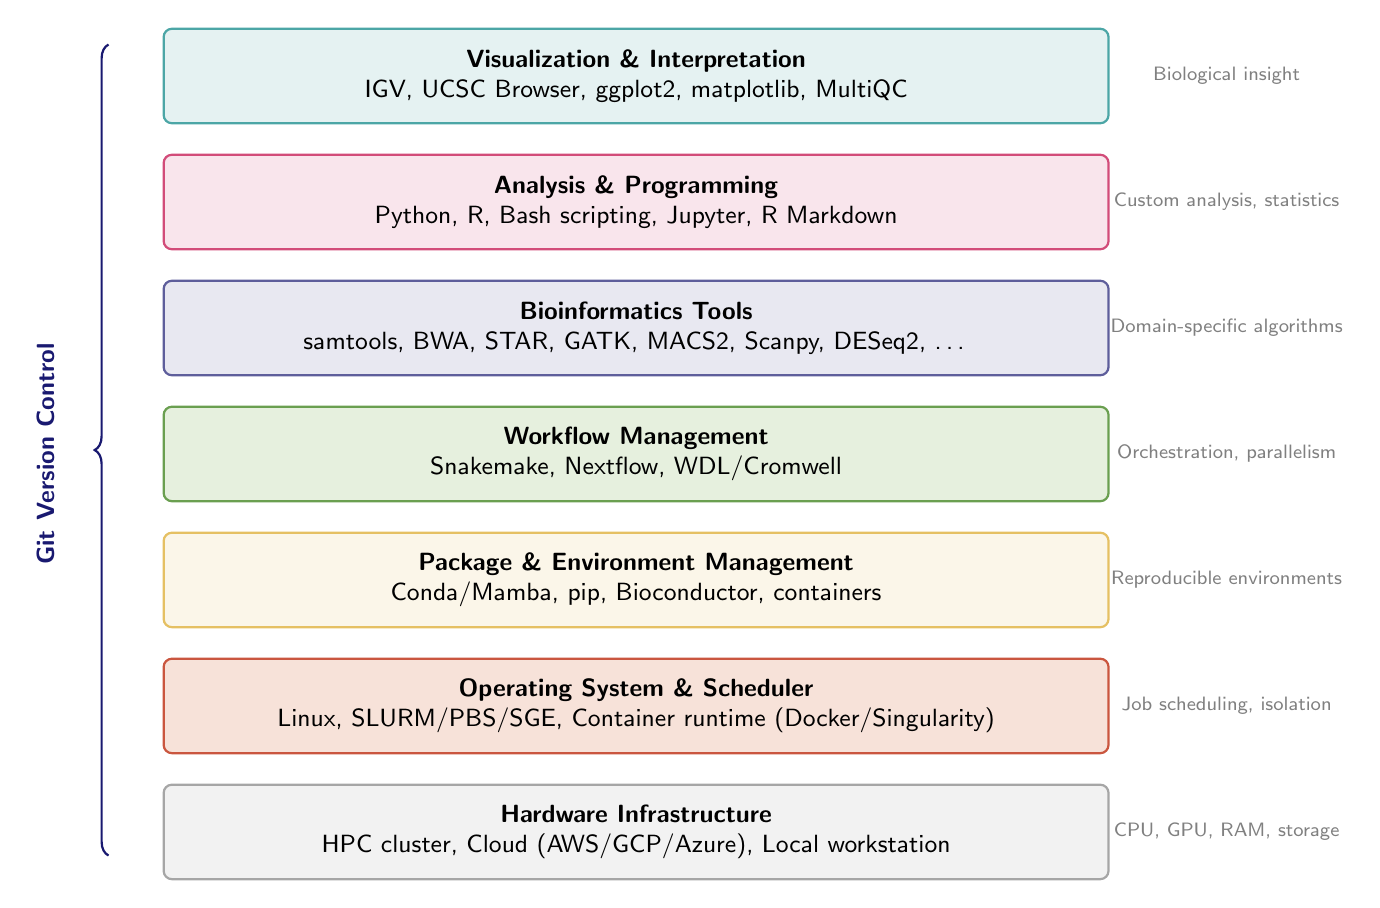
\begin{tikzpicture}[
  layer/.style={
    draw=#1!70, fill=#1!10, rounded corners=3pt,
    minimum width=12cm, minimum height=1.2cm,
    font=\sffamily\small, align=center, thick
  },
  note/.style={font=\scriptsize\sffamily, text=gray, align=left},
  arr/.style={-{Stealth[length=2.5mm]}, thick, gray!60}
]

% Stack layers from bottom to top
\node[layer=gray]        (hw)   at (0,0)    {\textbf{Hardware Infrastructure}\\HPC cluster, Cloud (AWS/GCP/Azure), Local workstation};
\node[layer=BrickRed]    (os)   at (0,1.6)  {\textbf{Operating System \& Scheduler}\\Linux, SLURM/PBS/SGE, Container runtime (Docker/Singularity)};
\node[layer=Goldenrod]   (pkg)  at (0,3.2)  {\textbf{Package \& Environment Management}\\Conda/Mamba, pip, Bioconductor, containers};
\node[layer=OliveGreen]  (wf)   at (0,4.8)  {\textbf{Workflow Management}\\Snakemake, Nextflow, WDL/Cromwell};
\node[layer=MidnightBlue](tool) at (0,6.4)  {\textbf{Bioinformatics Tools}\\samtools, BWA, STAR, GATK, MACS2, Scanpy, DESeq2, \ldots};
\node[layer=purple]      (lang) at (0,8.0)  {\textbf{Analysis \& Programming}\\Python, R, Bash scripting, Jupyter, R~Markdown};
\node[layer=teal]        (viz)  at (0,9.6)  {\textbf{Visualization \& Interpretation}\\IGV, UCSC Browser, ggplot2, matplotlib, MultiQC};

% Vertical labels on the right
\node[note] at (7.5, 0)   {CPU, GPU, RAM, storage};
\node[note] at (7.5, 1.6) {Job scheduling, isolation};
\node[note] at (7.5, 3.2) {Reproducible environments};
\node[note] at (7.5, 4.8) {Orchestration, parallelism};
\node[note] at (7.5, 6.4) {Domain-specific algorithms};
\node[note] at (7.5, 8.0) {Custom analysis, statistics};
\node[note] at (7.5, 9.6) {Biological insight};

% Side label: Version control spans all
\draw[decorate, decoration={brace, amplitude=5pt}, thick, MidnightBlue]
  (-6.7, -0.3) -- (-6.7, 10.0);
\node[rotate=90, font=\sffamily\small\bfseries, MidnightBlue] at (-7.5, 4.8) {Git Version Control};

\end{tikzpicture}
\caption[Bioinformatics computing stack.]{The layers of a modern bioinformatics computing stack. Version control (Git) spans all layers. Reproducibility requires attention at every level---from pinning software versions (environment management) to using workflow managers and containers.}
\label{fig:bioinfo-stack}
\end{figure}

%=============================================================================
\section{Summary}
\label{sec:bioinf:summary}
%=============================================================================

This chapter has introduced the foundational elements of bioinformatics that underpin all subsequent analysis chapters:

\begin{itemize}[itemsep=2pt]
  \item \textbf{Computing environment:} Linux command-line skills, package managers (Conda/Mamba), containers (Docker/Singularity), HPC clusters (SLURM), and cloud computing form the infrastructure layer.
  \item \textbf{File formats:} FASTA, FASTQ, SAM/BAM/CRAM, BED, GFF/GTF, VCF/BCF, BigWig, h5ad, and specialized formats for Hi-C and single-cell data are the lingua franca of bioinformatics.
  \item \textbf{Core tools:} samtools, bedtools, Picard, IGV, deepTools, and MultiQC are used in virtually every analysis pipeline.
  \item \textbf{Programming languages:} Python (with Biopython, pysam, Scanpy) and R (with Bioconductor, DESeq2, ggplot2) are complementary and both essential.
  \item \textbf{Workflow management:} Snakemake and Nextflow provide reproducibility, scalability, and portability for complex analysis pipelines. The nf-core community provides production-ready Nextflow pipelines.
  \item \textbf{Reproducibility:} Version control (Git), software version pinning, containers, workflow managers, and proper documentation are all essential for reproducible bioinformatics.
\end{itemize}

With these fundamentals in place, the next chapter presents complete, runnable analysis workflows for the major sequencing applications covered in this book.
